\documentclass{report}
\usepackage{graphicx} % Required for inserting images
\usepackage{booktabs} % For better horizontal lines
\usepackage{tabularx} % For width-adjustable tables
\usepackage{amsmath} % Math typesetting
\usepackage{gensymb} % Degree symbol
\usepackage{float} % To force table placement
\usepackage{setspace}    % To adjust line spacing

\begin{document}

\begin{titlepage}
    \centering

    \setstretch{1.5}
    {\Large \textbf{MACHINE LEARNING MODELS FOR PREDICTIVE ANALYSIS OF PRESSURE DROP AND TEMPERATURE IN POLYMER ELECTROLYTE MEMBRANE FUEL CELL STACKS TO FIND OPTIMAL FABRICATION PARAMETERS}}
    
    \vspace{5em}
    
    {\Large \textbf{HANHEE LEE}}
    
    \vfill
    
    {\Large ESROP GLOBAL}
    
    \vspace{1em} {\Large NATIONAL UNIVERSITY OF SINGAPORE}
    
    \vspace{1em} {\Large 2024}
    
\end{titlepage}

\pagenumbering{roman}

\begin{center}
    \section*{Declaration}
    I hereby declare that the thesis is my original work and it has been written by 
    me in its entirety. I have duly acknowledged all the sources of information 
    which have been used in this thesis. 
    
    \vspace{1em} \noindent This thesis has also not been submitted for any degree in any university previously 
    
    \vspace{1em} \noindent Hanhee Lee
    
    \vspace{1em} \noindent August, 2024
\end{center} 

\begin{center}
    \newpage \section*{Acknowledgements}
\end{center}
    \noindent I would like to express my sincere gratitude to Professor Erik Birgersson. Professor Birgersson has provided me with profound insights and knowledge on various topics, including polymer electrolyte membrane fuel cell stacks, machine learning, deep learning, and the use of COMSOL. He has also taught me how to effectively present to a scientific audience and the importance of learning independently. His enthusiasm and encouragement have made this journey a truly pleasant and enriching experience.

\begin{center}
    \newpage \section*{Abstract}    
\end{center}

\newpage \tableofcontents

\newpage \listoffigures

\newpage \listoftables

\newpage \section{List of Symbols}

    % Define custom column types with different proportional widths
    \newcolumntype{A}{>{\hsize=0.5\hsize}X} % Adjust these ratios as needed
    \newcolumntype{B}{>{\hsize=1.5\hsize}X}
    \newcolumntype{C}{>{\hsize=0.5\hsize}X}

    % Variables Table
    \begin{table}[h]
    \centering
    \begin{tabularx}{\textwidth}{ABC}
    \toprule
    \textbf{Name} & \textbf{Description} & \textbf{Unit} \\ 
    \midrule
    \( p \) & Pressure & Pa \\ 
    \( \mathbf{u}, \mathbf{U} \) & Velocity & m/s \\ 
    \( \rho \) & Density & kg/m$^3$ \\ 
    \( \mathbf{I} \) & Identity tensor & - \\ 
    \( \mathbf{K} \) & Viscous stress tensor & - \\ 
    \( \mathbf{F} \) & Volume force vector & - \\ 
    \( \mu \) & Dynamic viscosity & Pa$\cdot$s \\ 
    \( T \) & Temperature & K \\ 
    \( \mathbf{n} \) & Unit vector normal to the given surface & - \\ 
    \( \mathbf{G} \) & Reciprocal wall distance & - \\ 
    \( C_p \) & Specific heat capacity & J/(kg$\cdot$K) \\ 
    \( \mathbf{q} \) & Heat flux vector & - \\ 
    \( Q \) & Heat source & W/m$^3$ \\ 
    \( k \) & Thermal conductivity & W/(m$\cdot$K) \\ 
    \( R \) & Thermal resistance & (m$^2$$\cdot$K)/W \\ 
    \( d \) & Thin layer thickness & m \\ 
    \( \Delta \) & Delta & - \\ 
    \( \ell \) & Length/Distance & m \\ 
    \( u^+ \) & Tangential velocity in viscous units & - \\ 
    \( \sigma_w \) & Smoothing parameter & - \\ 
    Re & Reynolds number & - \\ 
    \( q \) & Quadratic loss coefficient & - \\ 
    \( \epsilon_p \) & Porosity & - \\ 
    \( \kappa \) & Permeability & m$^2$ \\ 
    \( \beta_F \) & Forchheimer coefficient & kg/m$^4$ \\ 
    \( Q_m \) & Mass source & kg/(m$^3$$\cdot$s) \\ 
    \bottomrule
    \end{tabularx}
    \caption{Variable Descriptions and Units}
    \label{tab:variables}
    \end{table}

    % Subscripts Table
    \begin{table}[H]
    \centering
    \begin{tabularx}{\textwidth}{AB}
    \toprule
    \textbf{Name} & \textbf{Description} \\ 
    \midrule
    \( 0 \) & Standard Conditions \\ 
    \( n \) & Unit vector normal to the given surface \\ 
    \( p \) & Point \\ 
    \( ted \) & Thermoelastic damping \\ 
    \( b \) & Boundary \\ 
    \( d \) & Down side \\ 
    \( s \) & Solid \\ 
    \( u \) & Up side \\ 
    \( ref \) & Reference \\ 
    \( w \) & Wall \\ 
    \( T \) & Turbulent \\ 
    \( exit \) & Exit \\ 
    \( pc \) & Pressure curve \\ 
    \bottomrule
    \end{tabularx}
    \caption{Subscript Descriptions}
    \label{tab:subscripts}
    \end{table}

    % Superscripts Table
    \begin{table}[H]
    \centering
    \begin{tabularx}{\textwidth}{AB}
    \toprule
    \textbf{Name} & \textbf{Description} \\ 
    \midrule
    \( T \) & Transpose \\ 
    \bottomrule
    \end{tabularx}
    \caption{Superscript Descriptions}
    \label{tab:superscripts}
    \end{table}

\pagenumbering{arabic}
\newpage \chapter{Introduction}
\section{Fuel Cells}
\newpage \chapter{Neural Networks}
\newpage \chapter{Literature Review}

\newpage \chapter{Materials and Methods}

    % Define custom column types with different proportional widths
    \newcolumntype{D}{>{\hsize=0.5\hsize}X} % Adjust these ratios as needed
    \newcolumntype{E}{>{\hsize=0.5\hsize}X}
    \newcolumntype{F}{>{\hsize=2.5\hsize}X}
    \newcolumntype{G}{>{\hsize=0.5\hsize}X}

    \newpage \begin{table}[H]
    \centering
    \begin{tabularx}{\textwidth}{DEFG} % Custom column widths
    \toprule
    \textbf{Header} & \textbf{Symbol} & \textbf{Explanation} & \textbf{Unit} \\ 
    \midrule
    \multicolumn{4}{c}{\textbf{Input Parameters}} \\
    \midrule
    Q & \( Q \) & \textbf{Heat generation} influences membrane hydration and operational efficiency; critical to prevent membrane dry-out and maintain ion conductivity. & \( \text{Wm}^{-2} \) \\
    Tamb & \( T_{amb} \) & \textbf{Ambient temperature of the air} sets baseline thermal conditions; higher temperatures boost performance to a limit before causing potential overheating. & \( \degree C \) \\
    Uin & \( U_{in} \) & \textbf{Airflow velocity} determines oxygen supply rate, essential for maintaining optimal reaction rates and power output. & \( \text{m/s} \) \\
    Wcc & \( W_{cc} \) & \textbf{Cathode channel width} determines oxygen flow and diffusion rates to the cathode, crucial for optimizing reaction efficiency. & \( \text{mm} \) \\
    Hcc & \( H_{cc} \) & \textbf{Cathode channel height} affects gas flow resistance and water removal, essential for maintaining membrane hydration and preventing flooding. & \( \text{mm} \) \\
    Lcc & \( L_{cc} \) & \textbf{Cathode channel length} influences the residence time of reactants and products along the channel, impacting overall fuel cell efficiency. & \( \text{mm} \) \\ 
    Wr & \( W_{r} \) & \textbf{Rib width} supports mechanical stability and maximizes the active area available for reactions, balancing structural support with performance. & \( \text{mm} \) \\
    Hr & \( H_{r} \) & \textbf{Rib height} controls the depth of flow channels, enhancing reactant distribution and efficient water management within the stack. & \( \text{mm} \) \\
    \midrule
    \multicolumn{4}{c}{\textbf{Output Performance Metrics}} \\
    \midrule
    Tsta & \( T_{stack} \) & \textbf{Stack temperature} is crucial for optimal reaction rates, membrane hydration, and to prolong the lifespan. & \( \degree C \) \\ 
    Delp & \( \Delta p \) & \textbf{Pressure drop} indicates the system's resistance to reactant flow; minimizing pressure drop is essential to enhance efficiency and ensure uniform distribution. & \( \text{Pa} \) \\ 
    \bottomrule
    \end{tabularx}
    \caption{Detailed Explanation of Variables}
    \end{table}
    
\chapter{COMSOL Model}
    \section{Model Assumptions}
        \begin{enumerate}
            \item The airflow entering the channel is turbulent. The Reynolds number exceeds 2300 at an inlet velocity ($U_{in}$) of 0.3 m/s.
            \item Portions of the fuel cell not part of the cathode flow field are impermeable to air. While carbon paper is porous, the in-plane pressure drop is much greater than that of the cathode flow field.
            \item The cathode flow field channels are modeled with a uniform height. The average offset (0.025 mm) is negligible compared to the channel height (1 mm).
            \item Cathode flow fields are modeled with straight edges and right-angle folds. The fold radius (0.05 mm) is small compared to the channel width (1 mm).
            \item Conservation of mass and momentum of airflow is assumed to be valid when transitioning between open spaces and cathode channels.
            \item A representative unit cell approximates the entire stack, excluding edge effects near the terminals. Airflow entering the unit cell is uniform and symmetrical.
            \item Channels are identical throughout the stack, resulting in no pressure drop differences between channels.
            \item The channels are fully dry without condensation. The oxidant stoichiometry exceeds 100, ensuring water vapor produced is absorbed by the airflow, negating the need for accounting water saturation.
            \item The losses from the fuel cell operation are converted to heat. 
        \end{enumerate}

        \section{Workflow - Pressure Drop}
        The following steps outline the workflow process for the unit cell simulations conducted in COMSOL:

        \begin{enumerate}
            \item \textbf{Selection of Laminar Flow Model:}
            \begin{itemize}
                \item This model was chosen because the airflow within the channels is laminar and is the largest contributor to the pressure drop across the stack.
                \item The laminar flow model allows for faster convergence and has been shown to be accurate when compared with experimental results.
            \end{itemize}
            
            \item \textbf{Construction of Unit Cell:}
            \begin{itemize}
                \item The unit cell was constructed using blocks with dimensions defined by equations to accommodate dimensional changes in the channels.
            \end{itemize}
            
            \item \textbf{Meshing Strategy:}
            \begin{itemize}
                \item A custom mesh was employed, focusing on the transition areas between inflow and outflow within the channels with a finer mesh.
                \item A coarser mesh was used within the channel and the air space between inflow and outflow.
                \item A mesh independence study was performed during the mesh fine-tuning. The results are shown in Figure ?.
                \item The difference between the blue dash (custom meshing) and green dots (physics-based extra fine meshing) is less than 3\%, thus the blue dash mesh was selected for its speed and accuracy.
            \end{itemize}
            
            \item \textbf{Parameter Sweep Function:}
            \begin{itemize}
                \item The parameter sweep function was utilized to explore all possible combinations for each stack size.
            \end{itemize}
            
            \item \textbf{Exporting Simulation Data:}
            \begin{itemize}
                \item The inputs and outputs of the simulations were exported from COMSOL for further analysis.
            \end{itemize}
        \end{enumerate}

        \section{Workflow - Temperature Stack}
        The following steps outline the workflow process for the unit cell simulations conducted in COMSOL:

        \begin{enumerate}
            \item \textbf{Selection of Physics Models:}
            \begin{itemize}
                \item The unit cell simulations were done using laminar flow physics as well as heat transfer in laminar flow.
                \item The parameter sweep function was utilized to explore all possible combinations in the parameter space.
                \item This model was selected because the flow through the channel is laminar and the simulation focuses on heat transfer within the channels.
            \end{itemize}
            
            \item \textbf{Construction of Unit Cell:}
            \begin{itemize}
                \item The unit cell was constructed using blocks with dimensions defined by equations to accommodate dimensional changes in the channels.
            \end{itemize}
            
            \item \textbf{Heat Generation Simulation:}
            \begin{itemize}
                \item Heat generation was simulated as a boundary heat source placed at the cathode side of the membrane.
            \end{itemize}
            
            \item \textbf{Heat Conduction Values:}
            \begin{itemize}
                \item The heat conduction values for each layer in the fuel cell were obtained from various papers, as shown in Table 8-1.
            \end{itemize}
            
            \item \textbf{Meshing Strategy:}
            \begin{itemize}
                \item A mesh independence study was conducted during the fine-tuning of the mesh. The results are shown in Figure ?.
                \item The difference between the blue dash and green dots is less than 1.06\%, hence the blue dash mesh was selected for its speed and accuracy.
            \end{itemize}
            
            \item \textbf{Exporting Simulation Data:}
            \begin{itemize}
                \item The inputs and outputs of the simulations were exported from COMSOL for further analysis.
            \end{itemize}
        \end{enumerate}

    \newpage \section{Parameters}
    
        \begin{table}[h]
        \centering
        \begin{tabularx}{\textwidth}{X X X}
        \toprule
        \textbf{Name} & \textbf{Value} & \textbf{Unit} \\ 
        \midrule
        Cell Area & 0.005 & m$^2$ \\ 
        Cell Voltage & 0.6 & V \\ 
        Compression & 0.1 & - \\ 
        Current & 40 & A \\ 
        Hbp & 5$\times$10$^{-5}$ & m \\ 
        Hcc & 1.25$\times$10$^{-3}$ & m \\ 
        Hcp & 3.15$\times$10$^{-4}$ & m \\ 
        Hmem & 1.5$\times$10$^{-5}$ & m \\ 
        Kcp & 1.5 & W$\cdot$m$^{-1}$K$^{-1}$ \\ 
        Kmem & 0.1 & W$\cdot$m$^{-1}$K$^{-1}$ \\ 
        Lcc & 0.03 & m \\ 
        pRef & 1.0133$\times$10$^5$ & Pa \\ 
        Q & 5040 & W$\cdot$m$^{-2}$ \\ 
        Tamb & 293.15 & K \\ 
        Test & 25.2 & W \\ 
        Uin & 7.75 & m$\cdot$s$^{-1}$ \\ 
        Wcc & 0.001 & m \\ 
        Wr & 5$\times$10$^{-5}$ & m \\ 
        \bottomrule
        \end{tabularx}
        \caption{Parameter Values}
        \label{tab:parameters}
        \end{table}
    
    \section{Materials}
        % Superscripts Table
        \begin{table}[H]
        \centering
        \begin{tabularx}{\textwidth}{BA}
        \toprule
        \textbf{Name} & \textbf{Unit} \\ 
        \midrule
        \multicolumn{2}{c}{\textbf{Air}} \\
        \midrule
        Dynamic viscosity & \( \text{Pa} \cdot \text{s} \) \\ 
        Ratio of specific heats & - \\ 
        Heat capacity at constant pressure & \(\text{J} / (\text{kg} \cdot \text{K})\) \\ 
        Density & \(\text{kg} / \text{m}^{3}\) \\ 
        Thermal conductivity & \(\text{W} / (\text{m} \cdot \text{K})\) \\
        \midrule
        \multicolumn{2}{c}{\textbf{Carbon Paper}} \\
        Density & \(\text{kg} / \text{m}^{3}\) \\ % No value
        Heat capacity at constant pressure & \(\text{J} / (\text{kg} \cdot \text{K})\) \\ % No value
        Thermal conductivity & \(\text{W} / (\text{m} \cdot \text{K})\) \\
        \midrule
        \midrule
        \multicolumn{2}{c}{\textbf{Membrane}} \\
        Thermal conductivity & \(\text{W} / (\text{m} \cdot \text{K})\) \\
        \midrule
        \midrule
        \multicolumn{2}{c}{\textbf{Steel Grade 316L}} \\
        Density & \(\text{kg} / \text{m}^{3}\) \\ % No value
        Heat capacity at constant pressure & \(\text{J} / (\text{kg} \cdot \text{K})\) \\ % No value
        Thermal conductivity & \(\text{W} / (\text{m} \cdot \text{K})\) \\
        \midrule
        \bottomrule
        \end{tabularx}
        \caption{Material Descriptions}
        \end{table}

    
    \section{Laminar Flow}
        \subsection{Governing Equations}
            \begin{equation}
                \rho (\textbf{u} \cdot \nabla) \textbf{u} = \nabla \cdot \left[-p\textbf{I} + \textbf{K} \right] + \textbf{F} 
            \end{equation}
                \noindent where \(\rho\) is the density of air, \textbf{u} is the velocity vector, p is the pressure, \textbf{I} is the identity matrix, \textbf{K} is the viscous stress tensor, and \textbf{F} is the volume force vector.
            \begin{equation}
                \nabla \cdot (\rho \textbf{u})= 0 % The equation is different in the thesis
            \end{equation}
            \begin{equation}
                \textbf{K} = \mu (\nabla \textbf{u} + (\nabla \textbf{u})^T) - \frac{2}{3} \mu (\nabla \cdot \textbf{u})\textbf{I} % NOTE: The equation is different from the one in the thesis.
            \end{equation}
                where \textbf{\(\mu\)} is the dynamic viscosity of air. 
    
        \subsection{Initial Values}
            \begin{enumerate}
                \item Velocity field
                    \begin{equation}
                        \textbf{u} = \textbf{0}
                    \end{equation}
                \item Pressure
                    \begin{equation}
                        p = 0
                    \end{equation}
            \end{enumerate}

        \subsection{Boundary Conditions}
            \begin{enumerate}
                \item Wall (No slip)
                    \begin{equation}
                        \mathbf{u} = \mathbf{0}
                    \end{equation}
            
                \item Inlet (Velocity)
                    \begin{equation}
                        \mathbf{u} = -U_{0} \mathbf{n}
                    \end{equation}
                        where \(U_{0}\) is the initial velocity (i.e. normal inflow velocity) and \(\mathbf{n}\) is the unit normal vector. 
                
                \item Outlet (Pressure)
                    \begin{equation}
                        \left[-p\textbf{I} + \textbf{K} \right]\mathbf{n} = - \hat{p}_{0} \mathbf{n} % this equation is different from the one in the thesis.
                    \end{equation}
                    \begin{equation}
                        \hat{p_{0}} \leq p_{0}, \nabla \mathbf{G} \cdot \mathbf{n} = 0
                    \end{equation}
                        where \(\hat{p}_{0}\) is the estimated standard condition pressure, \(p_{0}=0\) is the standard condition pressure (i.e. suppress backflow), \(\mathbf{G}\) is the reciprocal wall distance. 
            
                \item Symmetry 
                    \begin{equation}
                        \mathbf{u} \cdot \mathbf{n} = 0
                    \end{equation}
                    \begin{equation}
                        \mathbf{K}_{n} - (\mathbf{K}_{n} \cdot \mathbf{n})\mathbf{n} = 0, \mathbf{K}_{n} = \mathbf{Kn}
                    \end{equation}
            \end{enumerate}
            
    \section{Heat Transfer}
        \subsection{Governing Equations - Solid}
            \begin{equation}
                \rho C_{p} \textbf{u} \cdot \nabla T + \nabla \cdot \textbf{q} = Q + Q_{ted}
            \end{equation}
                \noindent where \(C_{p}\) is the specific heat capacity of air, T is the temperature of air, \textbf{q} is the heat flux vector, Q is the heat source, and \(Q_{ted}\) is the thermoelastic damping heat source.
            \begin{equation}
                \textbf{q} = -k \nabla T
            \end{equation}
                \noindent where k is the thermal conductivity. 
            \begin{equation}
                Q = (1.23 - Operating\ Voltage) \times \frac{Fuel\ Cell\ Stack\ Current}{Cell\ Area}
            \end{equation}
                
        \subsection{Governing Equations - Fluid}
            \begin{equation}
                \rho C_{p} \textbf{u} \cdot \nabla T + \nabla \cdot \textbf{q} = Q + Q_{p} + Q_{vd} % I dont know what vd is.
            \end{equation}
            \noindent where \(Q_{p}\) is the point heat source.
            \begin{equation}
                \textbf{q} = -k \nabla T
            \end{equation}
        
        \subsection{Governing Equations - Thin Layer}
            \begin{equation}
                -\textbf{n}_{d} \cdot \textbf{q}_{u} = \frac{(T_{u} - T_{d})}{R_{s}} + \frac{1}{2} d_{s} Q_{s}
            \end{equation}
            \noindent where \(R_s\) is the thermal resistance, and \(d_s\) is the thin layer thickness. 
            \begin{equation}
                -\textbf{n}_{u} \cdot \textbf{q}_{u} = \frac{(T_{d} - T_{u})}{R_{s}} + \frac{1}{2} d_{s} Q_{s}
            \end{equation}
            \begin{equation}
                R_{s} = \frac{d_{s}}{k_{s}}
            \end{equation}
        
        \subsection{Initial Values}
            \begin{enumerate}
                \item Temperature
                    \begin{equation}
                        T = T_{amb}
                    \end{equation}
                    where \(T_{amb}\) is the initial ambient temperature.
            \end{enumerate}
    
        \subsection{Boundary Conditions}
            \begin{enumerate}
                \item Insulation
                    \begin{equation}
                        -\mathbf{n} \cdot \mathbf{q} = 0
                    \end{equation}
            
                \item Symmetry
                    \begin{equation}
                        -\mathbf{n} \cdot \mathbf{q} = 0
                    \end{equation}
            
                \item Boundary Heat Source
                    \begin{equation}
                        -\mathbf{n} \cdot \mathbf{q} = Q_b
                    \end{equation}
                    where \(Q_b\) is the boundary heat source.
                
                \item Outflow
                    \begin{equation}
                        -\mathbf{n} \cdot \mathbf{q} = 0
                    \end{equation}
            
                \item Inlet
                    \begin{equation}
                        T = T_{amb}
                    \end{equation}
            \end{enumerate}
    
    \section{Mesh}
    
    \section{Study}
        \subsection{Difference between External and Internal Sweep}
            An internal sweep involves varying parameters directly within the 
            simulation model itself. This type of sweep is integrated into the 
            simulation process, where the solver automatically adjusts the parameters 
            as part of its internal algorithm. Internal sweeps are typically used to 
            explore the parameter space of the model in a more automated and 
            controlled manner, often leveraging the solver's built-in capabilities 
            to iterate through different parameter values.

            
            \vspace{1em} \noindent An external sweep, on the other hand, involves varying parameters outside 
            of the simulation model. This is usually managed by an external script 
            or control mechanism that systematically modifies the input parameters, 
            runs the simulation for each set of parameters, and collects the results. 
            External sweeps provide more flexibility and control over the parameter 
            variations and can be useful for complex scenarios where the internal 
            capabilities of the solver might be limited.
        \subsection{Parametric Sweep}
            A parametric sweep is a systematic method used in simulations and computational 
            experiments to explore the effects of varying parameters within a defined range. 
            By adjusting one or more input parameters incrementally, researchers can observe 
            how changes influence the outcome, enabling a comprehensive analysis of the 
            system's behavior. This technique is essential for optimizing designs, 
            identifying critical factors, and understanding the sensitivity of the results 
            to different variables. Ultimately, parametric sweeps provide valuable insights 
            that drive informed decision-making and innovation.

            \begin{table}[h]
            \centering
            \begin{tabularx}{\textwidth}{X X X}
            \toprule
            \textbf{Name} & \textbf{Values} & \textbf{Unit} \\ 
            \midrule
            Hcc & 1 1.25 1.5 1.75 2 & \(\text{mm}\) \\ 
            Wcc & 0.5 0.75 1 1.25 1.5 & \(\text{mm}\) \\ 
            Lcc & 30 60 90 & \(\text{mm}\) \\ 
            \bottomrule
            \end{tabularx}
            \caption{Parameter Sweep Values for All Combinations}
            \end{table}
        \subsection{Auxilary Sweep}
            An auxiliary sweep is a computational technique used to study the influence
            of secondary parameters or variables that are not directly part of the main 
            parametric study. It involves varying these auxiliary parameters to 
            investigate their impact on the primary simulation or experiment results. 
            This approach helps in understanding the interactions and dependencies 
            between primary and auxiliary parameters, providing a deeper insight into 
            the system's overall behavior. Auxiliary sweeps are particularly useful in 
            complex models where multiple factors may indirectly affect the outcomes, 
            aiding in fine-tuning and enhancing the accuracy of simulations.

            \begin{table}[h]
            \centering
            \begin{tabularx}{\textwidth}{X X X}
            \toprule
            \textbf{Name} & \textbf{Values} & \textbf{Unit} \\ 
            \midrule
            Uin & 1 3.25 5.5 7.75 10 & \(\text{m}/\text{s}\) \\ 
            Q & 1272 3132 5040 & \(W/\text{m}^{-2}\) \\ 
            Tamb & -20 0 20 40 & \(\degree \text{C}\) \\ 
            \bottomrule
            \end{tabularx}
            \caption{Auxilary Sweep Values for All Combinations}
            \end{table}
        
        \section{Results}
            \subsection{Accumulated Probe Table: Set 1}
                \begin{enumerate}
                    \item Hcc (1 - hc)
                    \item Wcc (2 - wc)
                    \item Lcc (3 - length)
                    \item Tamb (4 - Tamb)
                    \item Q (5 - Q)
                    \item Uin (6 - Uin)
                    \item Delp (15 - Pressure (Pa), Pressure Probe 3)
                        \begin{figure}[H]
                            \centering
                            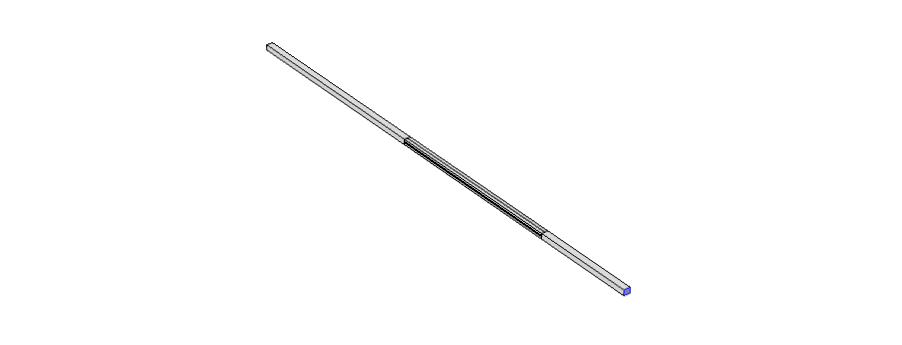
\includegraphics[width=0.75\textwidth]{00_Images/00_Pressure_Probe_3.png}
                            \caption{Pressure Probe 3 Location}
                        \end{figure}
                    \item Tsta (18 - Temperature (degC), Stack Temperature Probe 1)
                        \begin{figure}[H]
                            \centering
                            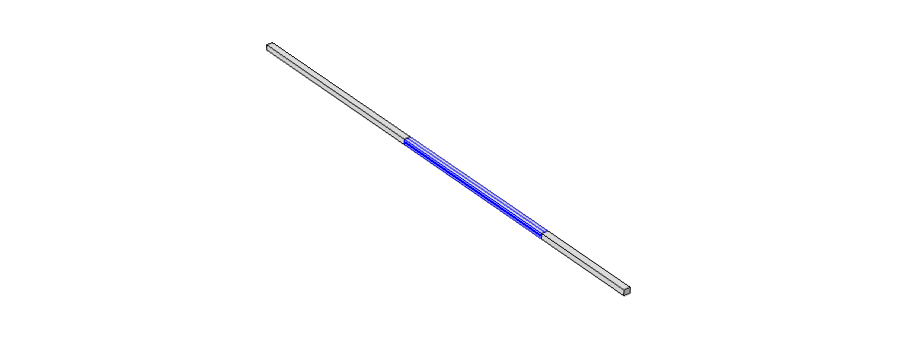
\includegraphics[width=0.75\textwidth]{00_Images/00_Stack_Temperature_Probe_1.png}
                            \caption{Stack Temperature Probe 1 Location}
                        \end{figure}
                \end{enumerate}

            \subsection{3D Plots}
                \begin{enumerate}
                    \item Pressure Drop
                        \begin{figure}[H]
                            \centering
                            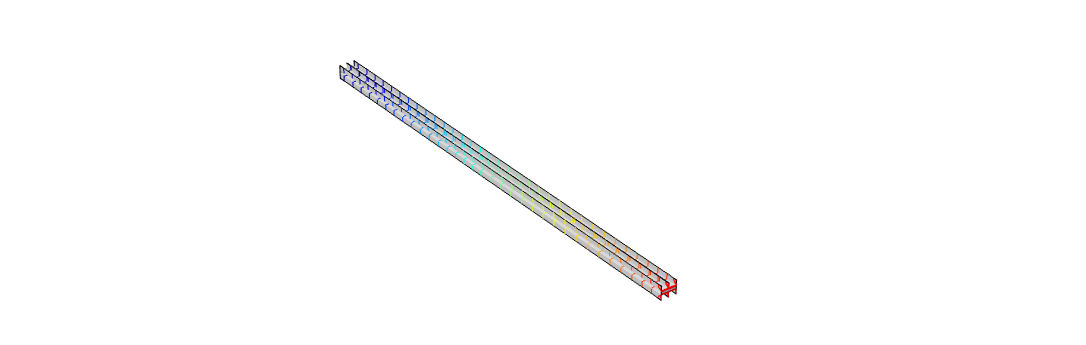
\includegraphics[width=0.75\textwidth]{00_Images/00_Pressure.png}
                            \caption{Pressure Drop 3D Plot}
                        \end{figure}
                    \item Temperature Stack
                        \begin{figure}[H]
                            \centering
                            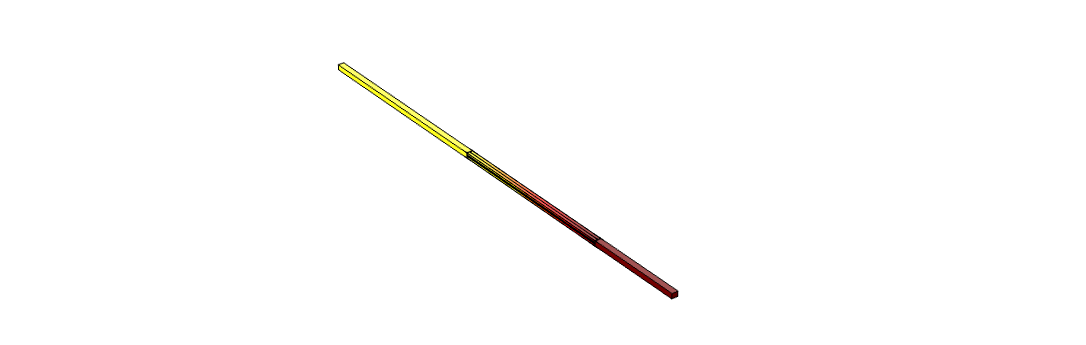
\includegraphics[width=0.75\textwidth]{00_Images/00_Temperature.png}
                            \caption{Temperature Stack 3D Plot}
                        \end{figure}
                    \item Velocity 
                        \begin{figure}
                            \centering
                            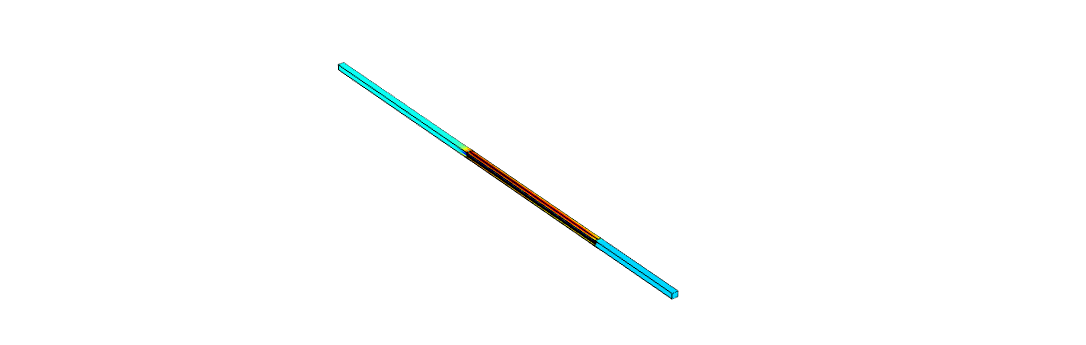
\includegraphics[width=0.75\textwidth]{00_Images/00_Velocity.png}
                            \caption{Velocity 3D Plot}
                        \end{figure}
                \end{enumerate}





\section{Conclusion}
\section{Outlook}
\section{References}

\end{document}
